
% File comsem.tex
%
%% Based on the style files for COLING-2014, which were, in turn,
%% Based on the style files for ACL-2014, which were, in turn,
%% Based on the style files for ACL-2013, which were, in turn,
%% Based on the style files for ACL-2012, which were, in turn,
%% based on the style files for ACL-2011, which were, in turn, 
%% based on the style files for ACL-2010, which were, in turn, 
%% based on the style files for ACL-IJCNLP-2009, which were, in turn,
%% based on the style files for EACL-2009 and IJCNLP-2008...

%% Based on the style files for EACL 2006 by 
%%e.agirre@ehu.es or Sergi.Balari@uab.es
%% and that of ACL 08 by Joakim Nivre and Noah Smith

\documentclass[11pt]{article}
\usepackage{coling2016}
\usepackage{times}
\usepackage{url}
\usepackage{latexsym}
\usepackage{graphicx}

%\setlength\titlebox{5cm}

% You can expand the titlebox if you need extra space
% to show all the authors. Please do not make the titlebox
% smaller than 5cm (the original size); I will check this
% in the camera-ready version and ask you to change it back.


\title{Instructions for Reports\\
       Computational Semantics LIX021M05}

\author{First Author \\
   Student Number \\
  {\tt email@domain} \\\And
  Second Author \\
   Student Number \\
  {\tt email@domain} \\}

\date{}

\begin{document}
\maketitle
\begin{abstract}
  This document contains the instructions for preparing reports
  required in the course LIX021M05 Computational Semantics. The
  document itself conforms to its own specifications, and is therefore
  an example of what your report should look like.  Students are asked
  to conform to all the directions reported in this document: a
  separate title page with abstract and table of contents, and the
  main text printed in double column format. 
\end{abstract}

\vfill
\tableofcontents
\clearpage 
\setcounter{page}{1}
\twocolumn

\section{Introduction}\label{sec:intro}

%
% The following footnote without marker is needed for the camera-ready
% version of the paper.
% Comment out the instructions (first text) and uncomment the 8 lines
% under "final paper" for your variant of English.
% 

The following instructions are directed to authors of reports
submitted for the computational semantics course. All students are
required to adhere to these specifications. Students are required to
provide a Portable Document Format (PDF) version of their papers and
upload these via Nestor. The aim of this document is to make it easier
to submit a report in the required format. 

This document contains first of all general formatting
constructions. If you use \LaTeX (strongly preferred), you can use
the source of this document as a starting point. Secondly, general
guidelines are given for writing your report.


\section{Formatting Instructions}

\subsection{Document Preparation}

It is strongly prefered that you prepare your PDF files using \LaTeX{} with
the official COLING 2016 style file (coling2016.sty) and bibliography
style (acl.bst). These files are available in report.zip in the
\textit{Course Resources} folder at Nestor.  You will also find the
document you are currently reading (comsem.pdf) and its \LaTeX{}
source code (comsem.tex) in this zip archive.  (You can alternatively
use Microsoft Word to produce your PDF file but this is not
recommended.)

For the production of the electronic manuscript you must use Adobe's
Portable Document Format (PDF). PDF files are usually produced from
\LaTeX{} using the \textit{pdflatex} command. If your version of
\LaTeX{} produces Postscript files, you can convert these into PDF
using \textit{ps2pdf} or \textit{dvipdf}. On Windows, you can also use
Adobe Distiller to generate PDF.  

Please make sure that your PDF file includes all the necessary fonts
(especially tree diagrams, symbols, and fonts with Asian characters).
If you cannot meet the above requirements for the production of your
electronic submission, please contact the the teacher of the course as
soon as possible.


\subsection{General Instructions}

Manuscripts must be in double-column format, except for the title
page.  The title, student name(s), and student number(s) must be
centred at the top of the first page (the title page). The title page
should also contain an abstract and a table of contents.  The title
page is not numbered. The page following the title should be
numbered page 1.


\subsection{Layout}
\label{ssec:layout}

Format manuscripts with a single column to a page, in the manner these
instructions are formatted. The exact dimensions for a page on A4
paper are shown in Table~\ref{table:sizes}.

\begin{table}[htbp]
\caption{\label{table:sizes} Dimensions.}
\begin{center}
\begin{tabular}{|l|r|}
\hline 
\bf Type & \bf Measure \\ 
\hline
\hline
Left and right margins &2.5 cm\\
 Top margin & 2.5 cm\\
Bottom margin& 2.5 cm\\
 Width& 16.0 cm\\
Height& 24.7 cm\\
\hline
\end{tabular}
\end{center}
\end{table}

\noindent Papers should not be submitted on any other paper size.
If you cannot meet the above requirements for
the production of your electronic submission, please contact the
teacher as soon as possible.


\subsection{Fonts}

For reasons of uniformity, Adobe's {\bf Times Roman} font should be
used. In \LaTeX2e{} this is accomplished by putting

\begin{quote}
\begin{verbatim}
\usepackage{times}
\usepackage{latexsym}
\end{verbatim}
\end{quote}
in the preamble. If Times Roman is unavailable, use {\bf Computer
  Modern Roman} (\LaTeX2e{}'s default).  Note that the latter is about
  10\% less dense than Adobe's Times Roman font.

\begin{table}[h]
\caption{\label{table:fonts} Font guide.}
\begin{center}
\begin{tabular}{|l|r|l|}
\hline 
\bf Type of Text & \bf Font Size & \bf Style \\ 
\hline
\hline
paper title & 15 pt & bold \\
author names & 12 pt & bold \\
the word ``Abstract'' & 12 pt & bold \\
section titles & 12 pt & bold \\
document text & 11 pt  &\\
captions & 11 pt & \\
sub-captions & 9 pt & \\
abstract text & 10 pt & \\
bibliography & 10 pt & \\
footnotes & 9 pt & \\
\hline
\end{tabular}
\end{center}
\end{table}

\subsection{Footnotes}

Put footnotes at the bottom of the page and use 9 pt
text. They may be numbered or referred to by asterisks or other
symbols.\footnote{This is how a footnote should appear.} Footnotes
should be separated from the text by a line.\footnote{Note the line
separating the footnotes from the text.}

\section{The Title Page}

The title page contains the title, name of the author(s), an abstract,
and a table of contents. It should not exceed one page.

\subsection{Title and Author}

Centre the title, author's name(s) and student number(s) across
the page.
Place the title centred at the top of the first page, in
a 15 pt bold font. (For a complete guide to font sizes and styles,
see Table~\ref{table:fonts}) Long titles should be typed on two lines
without a blank line intervening. Approximately, put the title at 2.5
cm from the top of the page, followed by a blank line, then the
author's names(s), and the student number on the following line. Do not
use only initials for given names (middle initials are allowed). 


\subsection{Abstract}

 Type the abstract between addresses and main body.
The width of the abstract text should be
smaller than main body by about 0.6 cm on each side.
Centre the word {\bf Abstract} in a 12 pt bold
font above the body of the abstract. The abstract should be a concise, informative
summary of the general thesis and conclusions of the paper. It should
be no longer than 200 words. The abstract text should be in 10 pt font.

\subsection{Table of Contents}

Include a table of contents on the title page. Do not include tables
of figures or tables.


\section{Main Parts}

\subsection{Sections}

The main body of the text should observing the double-column format as
shown in the present document and include page numbers.  Use 11 pt for
text and subsection headings, and 12 pt for section headings.  Type
and label section and subsection headings in the style shown on the
present document.  Use numbered sections (Arabic numerals) in order to
facilitate cross references. Number subsections with the section
number and the subsection number separated by a dot, in Arabic
numerals. Do not number subsubsections.

Usual sections of a report comprise an introduction, a section
describing related work and/or background, a section describing the
methodology used, a section reporting the results obtained, a section
discussing the results, and a conclusion. Hence, a typical structure
could be:

\begin{enumerate}
\item Introduction
\item Background and Related Work
\item Method and Data
\item Results and Discussion
\item Conclusion and Future Work
\end{enumerate}

Note that the first chapter, the introduction, should comprise the aim
of your research (motivation) and the specific objections that you
want to meet (the research questions).  The last chapter, the
conclusion, should provide answers to the research questions posed in
the introduction. The abstract should summarize the entire report, and
therefore should contain elements of all five parts shown above.


\subsection{Tables and Figures}

Place figures, tables, and photographs in the paper near where they
are first discussed, rather than at the end, if possible.  Colour
illustrations are discouraged, unless you have verified that they will
be understandable when printed in black ink. Figure~\ref{fig:geese}
illustrates how an image is included in a report.  Very wide figures
can be spread over the entire page width, as shown in
Figure~\ref{fig:wide}.

\begin{figure}[hbtp]
%\noindent\makebox[\linewidth]{\rule{\columnwidth}{1pt}}
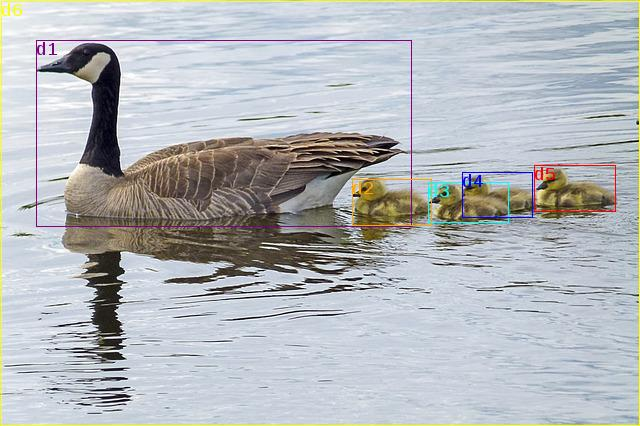
\includegraphics[width=\columnwidth]{canada-goose-436090_640_bb.jpg}
%\noindent\makebox[\linewidth]{\rule{\columnwidth}{1pt}}
\caption{A figure showing an image.\label{fig:geese}}
\end{figure}

\begin{figure*}[hbtp]
\scriptsize
\noindent\makebox[\linewidth]{\rule{\textwidth}{1pt}}
\begin{verbatim}
model([d1,d2,d3,d5,d6,d7],
      [f(1,n_woman_1,    [d1]),
       f(1,a_brown_1,    [d2]),
       f(1,n_hair_1,     [d2]),
       f(1,a_white_1,    [d3]),
       f(1,n_shirt_1,    [d3]),
       f(1,a_red_1,      [d5,d6]),
       f(1,n_apple_1,    [d6]),
       f(1,n_pear_1,     [d7]),
       f(1,n_lipstick_1, [d5]),
       f(2,s_part_of,    [(d2,d1)]),
       f(2,s_touches,    [(d1,d6),(d6,d1),(d1,d7),(d7,d1),(d1,d2),(d2,d1),(d1,d5),(d5,d1),(d1,d3),(d3,d1)]),
       f(2,s_supports,   [(d1,d3),(d1,d6),(d1,d7),(d1,d5)]),
       f(2,s_near,       [(d2,d1),(d3,d2),(d5,d1),(d6,d1),(d7,d1),(d1,d2),(d5,d2),(d1,d3),(d2,d3)])]).
\end{verbatim}
\noindent\makebox[\linewidth]{\rule{\textwidth}{1pt}}
\caption{A wide figure ranging over two columns.\label{fig:wide}}
\end{figure*}


Provide a caption for every illustration. Number each one sequentially
in the form: ``Figure 1. Caption of the Figure.''  ``Table 1.  Caption
of the Table.''  Type the captions of the figures \textit{below} the
body of the figure, and the captions of tables \textit{above} the body
of the table (as shown, for example, in Table~\ref{table:sizes} and
Table~\ref{table:fonts}), using 11 pt text.




\subsection{Citations and References}

 Citations within the text appear in parentheses
as~\cite{Bos2015NoDaLiDa} or, if the author's name appears in the text
itself, as Bos~\shortcite{Bos2015NoDaLiDa}.  Append lowercase letters
to the year in cases of ambiguity.  Treat double authors as
in~\cite{BlackburnBos2005CSLI}, but write as in~\cite{monroe-goodman-potts:2016:EMNLP2016} when more than two
authors are involved. Collapse multiple citations as
in~\cite{BlackburnBos2005CSLI,Bos2015NoDaLiDa}. Also refrain from using full citations
as sentence constituents. So instead of
\begin{quote}
  ``\cite{Bos2015NoDaLiDa} showed that ...''
\end{quote}
you should use:
\begin{quote}
   ``\newcite{Bos2015NoDaLiDa}   showed that ...''
\end{quote}

If you are using the provided \LaTeX{} and Bib\TeX{} style files, you
can use the command \verb|\newcite| to get ``author (year)'' citations.

Gather the full set of references together under
the heading {\bf References}; place the section before any Appendices,
unless they contain references. Arrange the references alphabetically
by first author, rather than by order of occurrence in the text.
Provide as complete a citation as possible, using a consistent format,
such as the one for {\em Computational Linguistics\/} or the one in the 
{\em Publication Manual of the American 
Psychological Association\/}.  Use of full names for
authors rather than initials is preferred.  
The \LaTeX{} and Bib\TeX{} style files provided roughly fit the
American Psychological Association format, allowing regular citations, 
short citations and multiple citations as described above.


\subsection{Appendices} 

Use an appendix for long tables, manuals, large figures, and extracts
of source code, that somehow do not fit on the main body of the
report.  Appendices should directly follow the text and the references
on a new page.  Letter them in sequence and provide an informative
title.

% include your own bib file like this:

\bibliographystyle{acl}
\bibliography{comsem}

% this is the place to include appendices:

\onecolumn
\appendix
\section{Source Code of $\alpha$-Conversion} \scriptsize
\noindent\makebox[\linewidth]{\rule{\textwidth}{1pt}}
\begin{verbatim}
:- module(alphaConversion,[alphaConvert/2,
                           alphabeticVariants/2]).

/*========================================================================
   Alpha Conversion (introducing substitutions)
========================================================================*/

alphaConvert(F1,F2):-
   alphaConvert(F1,[],[]-_,F2).

/*========================================================================
   Alpha Conversion 
========================================================================*/

alphaConvert(X,Sub,Free1-Free2,Y):-
   var(X), 
   (
      member(sub(Z,Y),Sub),
      X==Z, !,
      Free2=Free1
   ;
      Y=X,
      Free2=[X|Free1]
   ).

alphaConvert(Expression,Sub,Free1-Free2,some(Y,F2)):-
   nonvar(Expression),
   Expression = some(X,F1),
   alphaConvert(F1,[sub(X,Y)|Sub],Free1-Free2,F2).

alphaConvert(Expression,Sub,Free1-Free2,all(Y,F2)):- 
   nonvar(Expression),
   Expression = all(X,F1),
   alphaConvert(F1,[sub(X,Y)|Sub],Free1-Free2,F2).

alphaConvert(Expression,Sub,Free1-Free2,lam(Y,F2)):- 
   nonvar(Expression),
   Expression = lam(X,F1),
   alphaConvert(F1,[sub(X,Y)|Sub],Free1-Free2,F2).

alphaConvert(Expression,Sub,Free1-Free3,que(Y,F3,F4)):-
   nonvar(Expression),
   Expression = que(X,F1,F2),
   alphaConvert(F1,[sub(X,Y)|Sub],Free1-Free2,F3),
   alphaConvert(F2,[sub(X,Y)|Sub],Free2-Free3,F4).

alphaConvert(F1,Sub,Free1-Free2,F2):-
   nonvar(F1),
   \+ F1 = some(_,_),
   \+ F1 = all(_,_),
   \+ F1 = lam(_,_),
   \+ F1 = que(_,_,_),
   F1 =.. [Symbol|Args1],
   alphaConvertList(Args1,Sub,Free1-Free2,Args2),
   F2 =.. [Symbol|Args2].

/*========================================================================
   Alpha Conversion (listwise)
========================================================================*/

alphaConvertList([],_,Free-Free,[]).

alphaConvertList([X|L1],Sub,Free1-Free3,[Y|L2]):-
   alphaConvert(X,Sub,Free1-Free2,Y),
   alphaConvertList(L1,Sub,Free2-Free3,L2).

/*========================================================================
   Alphabetic Variants
========================================================================*/

alphabeticVariants(Term1,Term2):-
   alphaConvert(Term1,[],[]-Free1,Term3),
   alphaConvert(Term2,[],[]-Free2,Term4),
   Free1==Free2,
   numbervars(Free1,0,N),
   numbervars(Term3,N,M),
   numbervars(Term4,N,M),
   Term3=Term4.
\end{verbatim}
\noindent\makebox[\linewidth]{\rule{\textwidth}{1pt}}


\end{document}
